\section{Problems}
\label{ssec:testHWprobs}
Unfortunately, at the point of testing a few issues became apparent.
The first of these was a footprint error.
Due to an error in design the footprint for the OP-AMPs was set to TSOP8, whereas the actual footprint of the component was SOP8.
These footprints are so significantly different there was no way to make the components use the footprint, as such they were unpopulated.
An alternative was sourced, however time and cost constraints prevented them actually being put to use.
\\
\\
The next problem to be discovered was that the fact that the DSP had no on-board flash had not been accounted for.
This was not a major issue as the DSP is capable of running from code in the RAM.
However, actually programming the flash was also an issue.
Both urJTAG and OpenOCD were experimented with, neither with much success.
After a short amount of time it was decided that fighting with the programming capabilities were secondary to getting the algorithm working, and as time was limited it was decided to leave the programming, and come back to it at a later date if time presented itself.
\\
\\
To begin with there was also a short in the power management section.
This was discovered to be a misinterpretation of the pin out of the voltage regulators, resulting in the output voltage being connected directly to the ground plane through the additional pin.
This issue was solved by removing the tracks between the pad for that pin, and the ground plane.

\section{Test Conditions}
\label{ssec:testHWconds}
The test conditions as shown in table \ref{tab:testconditions} were used for all the tests unless otherwise stated.

\begin{table}[H]
	\centering
	\begin{tabular}[c]{| l | l | c |}
		\hline
		\multicolumn{2}{|l|}{Factor}		& Value	\\
		\hline
		\multicolumn{2}{|l|}{Voltage}		& 5.00V	\\
		\multicolumn{2}{|l|}{Current Limit}	& 800mA	\\
		\hline
		\multirow{4}{*}{J105}	& $DV_{dd}$	& Unconnected	\\
					& $CV_{dd}$	& Unconnected	\\
					& Codec		& Unconnected	\\
					& Amp		& Unconnected	\\
		\hline
		\multirow{4}{*}{J106}	& Right		& Unconnected	\\
					& Middle Right	& Unconnected	\\
					& Middle Left	& Unconnected	\\
					& Left		& Unconnected	\\
		\hline
		\multirow{4}{*}{J107}	& Right		& Unconnected	\\
					& Middle Right	& Unconnected	\\
					& Middle Left	& Unconnected	\\
					& Left		& Unconnected	\\
		\hline
		\multirow{4}{*}{J108}	& Right		& Unconnected	\\
					& Middle Right	& Unconnected	\\
					& Middle Left	& Unconnected	\\
					& Left		& Unconnected	\\
		\hline
		\multicolumn{2}{|l|}{CONN401}		& Unconnected	\\
		\hline
	\end{tabular}
	\caption{The conditions used in testing}
	\label{tab:testconditions}
\end{table}

\subsection{DSP}
\begin{table}[H]
	\centering
	\begin{tabular}[c]{| l | l | c |}
		\hline
		\multicolumn{2}{|l|}{Factor}		& Value	\\
		\hline
		\multirow{4}{*}{J105}	& $DV_{dd}$	& Connected	\\
					& $CV_{dd}$	& Connected	\\
					& Codec		& -		\\
					& Amp		& -		\\
		\hline
	\end{tabular}
	\caption{Conditions for testing the DSP}
	\label{tab:dsptestconditions}
\end{table}

\subsection{Codec}
\begin{table}[H]
	\centering
	\begin{tabular}[c]{| l | l | c |}
		\hline
		\multicolumn{2}{|l|}{Factor}		& Value	\\
		\hline
		\multirow{4}{*}{J105}	& $DV_{dd}$	& -		\\
					& $CV_{dd}$	& -		\\
					& Codec		& Connected	\\
					& Amp		& -		\\
		\hline
	\end{tabular}
	\caption{Conditions for testing the Codec}
	\label{tab:codectestconditions}
\end{table}


\subsection{Analogue}
\begin{table}[H]
	\centering
	\begin{tabular}[c]{| l | l | c |}
		\hline
		\multicolumn{2}{|l|}{Factor}		& Value	\\
		\hline
		\multirow{4}{*}{J105}	& $DV_{dd}$	& -		\\
					& $CV_{dd}$	& -		\\
					& Codec		& -		\\
					& Amp		& Connected	\\
		\hline
	\end{tabular}
	\caption{Conditions for testing the signal conditioning amplifier}
	\label{tab:analoguetestconditions}
\end{table}

\section{Results}
\label{ssec:testHWresults}
\subsubsection{Power}
This circuitry was tested by connecting a bench power supply to the voltage inputs, and measuring the output voltage from the regulators using a digital oscilloscope.
Table \ref{tab:powisotest} shows the results.
The voltage level on the external side of the header was also tested, to check that power wasn't being shorted across.

\begin{table}[H]
	\centering
	\begin{tabular}[c]{| l | c | c |}
		\hline
		Conn		& VR Out (V)	& SC Pin (mV)	\\
		\hline
		$DV_{dd}$	& 3.28		& 190		\\
		$CV_{dd}$	& 1.21		& 37		\\
		Codec		& 3.28		& 34		\\
		Amp		& 3.28		& 32		\\
		\hline
	\end{tabular}
	\caption{The voltages provided by the power circuitry}
	\label{tab:powisotest}
\end{table}

\noindent These results show that the desired voltages were produced.
There was clearly some noise on the external side of the system, however this was low enough to not power up any of the devices.
\\
\\
Another important part of this test was the LED to indicate when the system was powered.
For as long as power was provided to the system this LED stayed lit, as desired.


\subsubsection{DSP}
One test that was possible was simply to power up the DSP, both core and I/O, and check that there were no short circuits.
The conclusion of this test was simply that there were no short circuits, as the power supply did not current limit.
\\
\\
Another possible test was the functionality of the JTAG port.
This was tested by attempting to read the device ID over JTAG.
Two functions were run under urJTAG, the first being an attempt to detect the JTAG chain, the second to fetch and recognise the ID code.
\\
\\
The result from running `detect' is show below:
\\
\\
\emph{
\indent jtag$>$ detect	\\
\indent IR  length: 46	\\
\indent Chain length: 1	\\
\indent Device Id: 0 (0x0000000000000000)	\\
\indent chain.c(149) Part 0 without active instruction	\\
\indent chain.c(200) Part 0 without active instruction	\\
\indent chain.c(149) Part 0 without active instruction	\\
}

\noindent As the IR length documented for this DSP is 46, this shows a valid detection of the device in the chain, however detection of the ID code failed.
A similar effect is seen from the result of `idcode':
\\
\\
\emph{
\indent jtag$>$ idcode	\\
\indent Reading 0 bytes if idcode	\\
\indent Read 00000000 00000000 00000000 00000000	\\
}

\noindent This shows that the device ID was undetectable.
\subsubsection{Codec}
When tested, the output of the clock generator produced the waveform in figure \ref{fig:codec12Mclk}.
This shows that the clock generator was producing a $12MHz$ square wave signal as desired.
This signal was between $0-3.3V$ as required by the codec inputs, however reached $5V_{pk-pk}$ which would not have been acceptable by the codec.
In order to resolve this issue a small capacitor could be placed in parallel with the output of the clock generator.
This would serve the purpose of removing the ripples on the signal and keep it within the bounds required by the codec.

\begin{figure}[H]
	\centering
	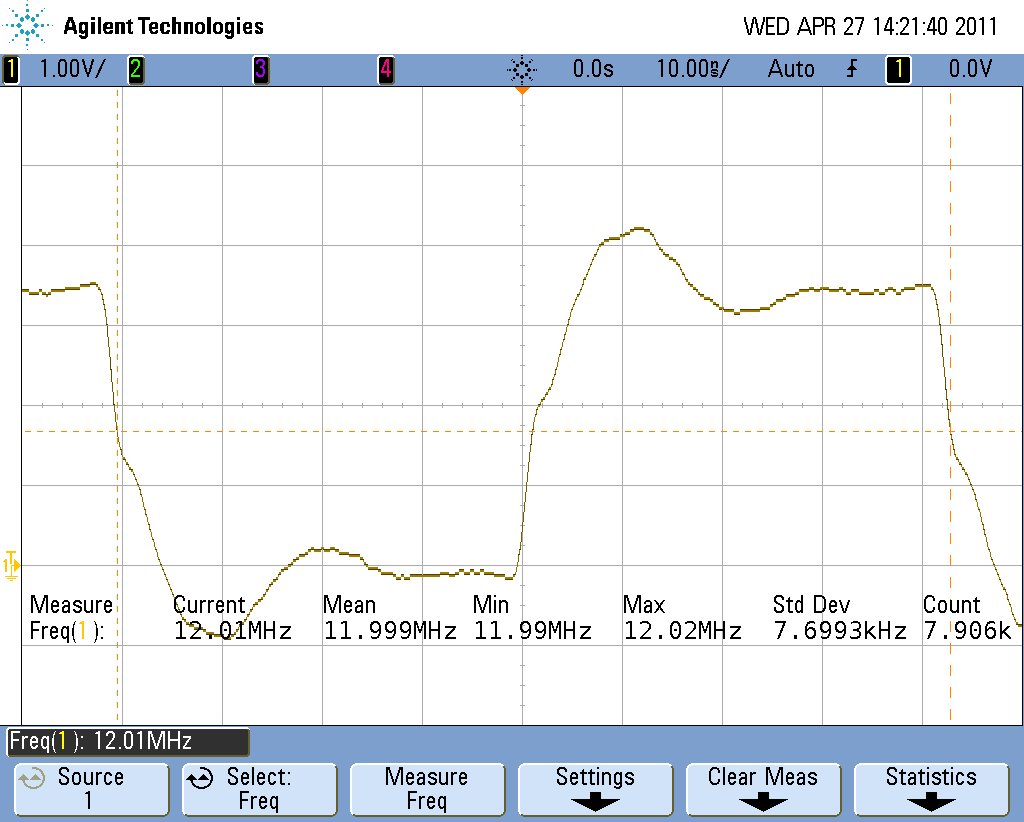
\includegraphics[width=\textwidth]{./img/codec_12M_clk.png}
	\caption{Output waveform of the clock generator}
	\label{fig:codec12Mclk}
\end{figure}

\subsubsection{Analogue}
A sine wave at 5.03V peak to peak was applied at the input of one of the signal conditioners, and an oscilloscope probe connected to the output.
The frequency of the input sine wave was then changed and the output peak to peak voltage measured at each frequency.
This resulted in the graph shown by figure \ref{fig:sigcondtest}.
This graph shows that the response of the amplifier matches the simulation (figure \ref{fig:sigcondmodel}).
Therefore the signal conditioning amplifier performs as expected.
\\
\\

\begin{sidewaysfigure}
	\centering
	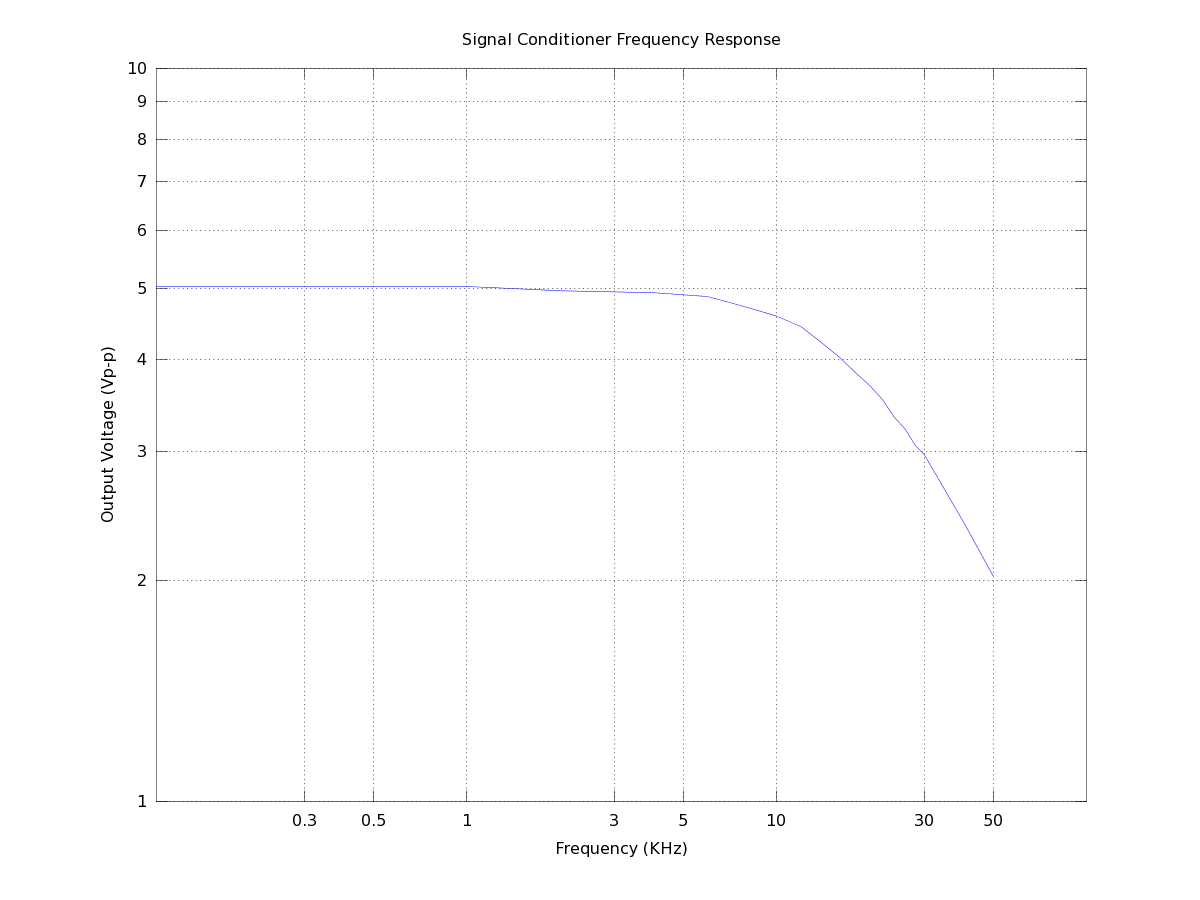
\includegraphics[width=\textwidth]{./img/sigcondtest.png}
	\caption{The frequency response of the signal conditioning amplifier}
	\label{fig:sigcondtest}
\end{sidewaysfigure}

\noindent The instrumentation amplifier was not populated due to a footprint error, therefore it was not tested.

\section{LMS}
\label{ssec:testSWlms}
\subsubsection{Linux}
A sine wave was generated taking only integer values between $0$ and $2000$.
This was to emulate the effect of the codec, which returns only integer values.
The codec code was replaced in order to read in each of these values in turn, and to return them in such a way that they could be treated as both the noise signal and the heard signal.
\\
\\
The code was then run.
As each output value was calculated it was saved to a file, allowing the values to be loaded into Matlab.
These output values could then be plotted.
The code was run twice, once saving the output, and again saving the error.
The results of each of these can be seen in figures \ref{fig:testlmslinuxout} and \ref{fig:testlmslinuxerr} respectively.

\begin{figure}[H]
	\centering
	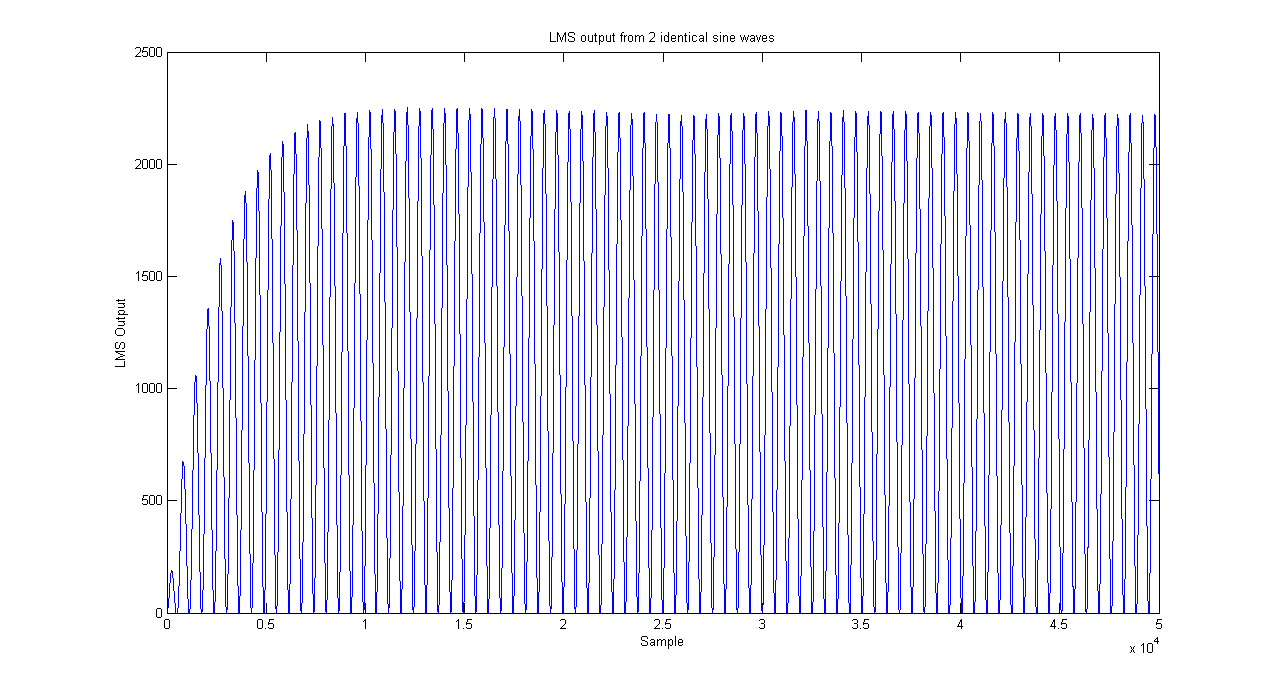
\includegraphics[width=\textwidth]{./img/lms_linux_out.png}
	\caption{The LMS Output from Linux terminal simulation}
	\label{fig:testlmslinuxout}
\end{figure}

\noindent These figures show that the LMS code is functioning as desired, reaching an attenuation of $17dB$ before reaching the end of the samples.

\begin{figure}[H]
	\centering
	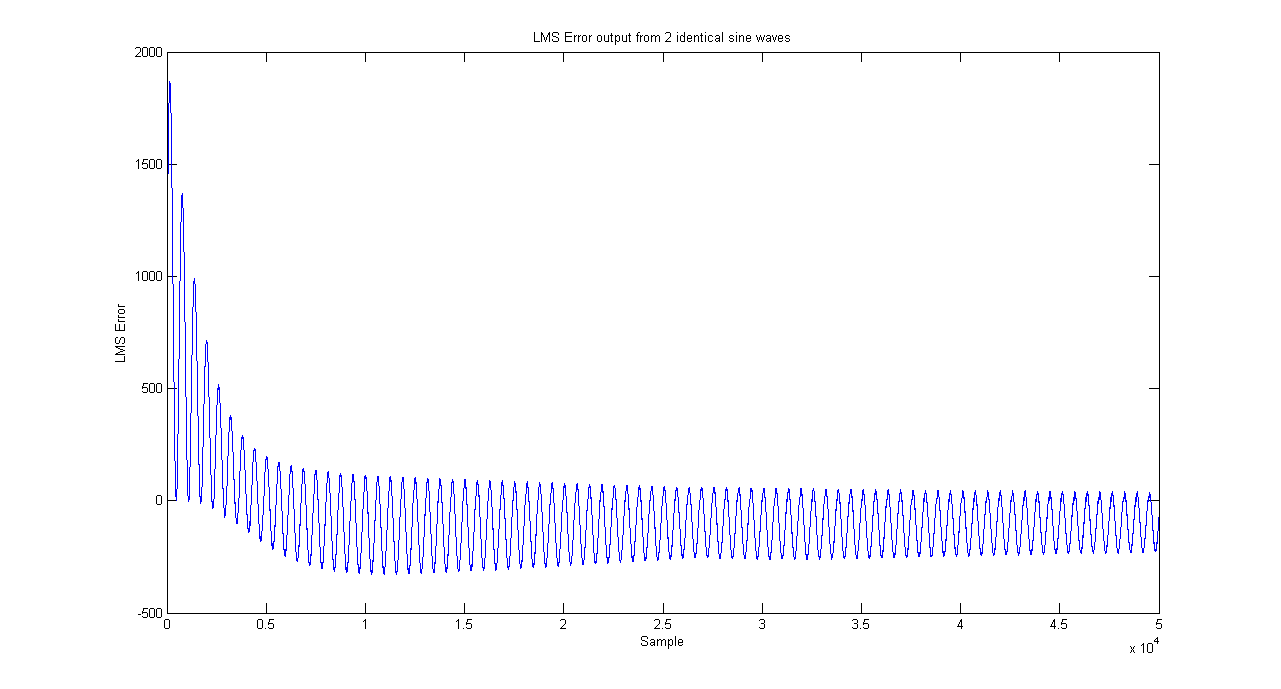
\includegraphics[width=\textwidth]{./img/lms_linux_err.png}
	\caption{The LMS Error from Linux terminal simulation}
	\label{fig:testlmslinuxerr}
\end{figure}

\subsubsection{DSP}
The code was loaded onto the DSP evaluation board.
Like the correlation method, the code did not run fast enough, reaching a frequency of approximately $7.5KHz$.
This is approximately 6 times too slow.

